\documentclass[english]{cgspaper} % change option to 'english' to include english logo in \copyrightspace

%\usepackage[ngerman]{babel} % comment out to use english in auto-generated section titles
\usepackage[utf8]{inputenc}
\usepackage[ruled]{algorithm}
\usepackage{algpseudocode}
\usepackage[hyphens]{url}
\usepackage{csquotes}
\usepackage{subcaption}
\usepackage{hyperref}

%\usepackage[backend=biber,style=authoryear, citestyle=authoryear]{biblatex}
%\addbibresource{foo-paper.bib}

\title{Demonstration of Game-Based Object Detection}
\author{
    Tom Beckmann, Philipp Bode,\\ Julius C. R. Rudolph, Hendrik Rätz\\ Digital Engineering Faculty, Hasso Plattner Institute \textbar{} University of Potsdam
}
% \author{}
% \author{Julius C. R. Rudolph\\ Digital Engineering Faculty, Hasso Plattner Institute \textbar{} University of Potsdam}
% \author{Hendrik Rätz\\ Digital Engineering Faculty, Hasso Plattner Institute \textbar{} University of Potsdam}

% Konfiguration des Veranstaltungs-Feldes
\subject{%
    \textbf{Advanced Games of Life}\\
    Sommersemester 2018\\
    Themenstellung und Anleitung:
    Daniel Limberger und Prof.\ Dr.\ Jürgen Döllner}

\begin{document}

% Definition des Teasers
%\teaser{
    %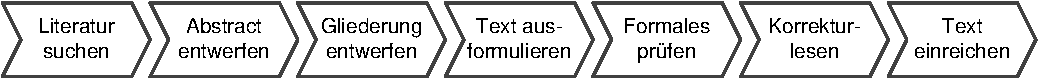
\includegraphics[width=0.9\textwidth]{graphics/prozess.pdf}
    %\caption{Beispiel für einen Teaser: Schritte beim Erstellen eines fachwissenschaftlichen Beitrags. Ein Teaser dient als Blickfang schon auf der ersten Seite eines Artikels.}
    %\label{fig:prozess}
%}

\maketitle


%----------------------------------------------------------------
% Zusammenfassung
%----------------------------------------------------------------
\begin{abstract}
With the emergence of easy-to-use Augmented Reality (AR) frameworks and increasing capabilities of modern smartphones, the potential for automated analysis of the user's camera feed arises.
However, malicious actors could employ such analyses for illicit surveillance or unethical profiling use cases, all the while staying hidden from the end user.
We propose a showcase application that demonstrates two of these use cases. In the context of an AR game, we scan the user's perimeter for brand logos and try to lead the player into providing close-up shots of potentially sensitive textual information.
Even though the app is prototypical, through it one can foresee the severe potential for misuse of soon-to-be widespread AR applications.
\end{abstract}

\copyrightspace % Erzeugt den Hinweis auf die Veranstaltung links unten
%----------------------------------------------------------------
% Introduction
%----------------------------------------------------------------
\section{Introduction}
- features of today's smartphones 
 - cameras able to take high resolution pictures/videos
 - geolocation via GPS
 - ability to use high speed internet (where available) -> send high amounts of data/video streaming possible
 - high processing power, multiple cores, quite some RAM
 - allows complex calculations, analysis of video data, e.g. in context of AR

- Pokemon-Go
- popular game about catching Pokemon in the real world
- around 800 million downloads (30.5.18, https://www.playm.de/2018/05/pokemon-go-35-403807/)

- uses location of user to identify Pokemon/Events/special places near him
- able to use AR to interact with Pokemon in real world 
- (always) connected to the internet and able to transfer data, no opt-out

- possible to create very detailed profiles of players
- tracking of location and movement (further analysis could discover certain habits/patterns)
- analysis of everything where persons points their camera at: texts, faces, brands
- can be used for espionage, preparation of crimes or simply targeted advertisements

- hence we created a demo showcase to reveal the potential dangers that the improvident usage of AR-apps can bring

%%----------------------------------------------------------------
% Lehrstuhlkontext: 
% Diesen Abschnitt (in der deutschen bzw. englischen Fassung) übernehmen 
%----------------------------------------------------------------

%\section{Kontext}
%\label{sec:Kontext}
%Die Betreuung im Rahmen der Seminartätigkeit erfolgte durch das Fachgebiet für Computergrafische Systeme, dessen Forschungsschwerpunkt die Prozessierung, Abbildung und interaktive Visualisierung massiver raumzeitlicher \cite{Oehlke2015,Buschmann2015,Buschmann2014,Maass2006} sowie abstrakter, hochdimensionaler Daten \cite{Limberger2017,Limberger2016,Wuerfel2015} ist. Dies beinhaltet neben neuartigen Algorithmen \cite{RichterKyprianidis2013,RichterBehrens2013,Glander2012}, Rendering-Techniken \cite{Semmo2016,Pasewaldt2014,Maass2006a,Doellner2005} und Interaktions-Metaphern \cite{Semmo2016a,Scheibel2016,Semmo2014} auch effiziente Datenstrukturen \cite{Scheibel2017,Richter2015} und Systemarchitekturen \cite{Klimke2014,Trapp2012,Klimke2010}, die anhand von real-weltlicher Datensätze und Anwendungsszenarien  \cite{Discher2016,Trapp2015,Engel2012} evaluiert werden. 

\section{Context}
\label{sec:Context}
This course project was supervised by the Computer Graphics Systems Group whose main research interest includes the processing, mapping, and interactive visualization of massive spatio-temporal information \cite{Oehlke2015,Buschmann2015,Buschmann2014,Maass2006} and abstract high-dimensional information \cite{Limberger2017,Limberger2016,Wuerfel2015}. In particular, this comprises novel algorithms \cite{RichterKyprianidis2013,RichterBehrens2013,Glander2012}, rendering techniques \cite{Semmo2016,Pasewaldt2014,Maass2006a,Doellner2005}, and interaction metaphors \cite{Semmo2016a,Scheibel2016,Semmo2014}, as well as efficient data structures \cite{Scheibel2017,Richter2015} and system architectures \cite{Klimke2014,Trapp2012,Klimke2010} which are evaluated based on real-world data sets and application scenarios \cite{Discher2016,Trapp2015,Engel2012}.



% Wie analysieren wir diese?

%----------------------------------------------------------------
% Concept
%----------------------------------------------------------------
\section{Privacy intrusion through AR and CV technologies}

-(factor 1) Advancement of augmented reality technologies (robustness, accuracy) and ease of integration (AR libraries) will presumably lead to a surge in mobile applications utilizing such features. \\
-(factor 2) Current AR applications are often developed for entertainment purposes or as feature showcase, but with increasing maturity of the technology, conceivable use cases appear in a wide range of domains, e.g. information display in professional environments, medical application, support of sensory functions, etc. \\
- (factor 3) By necessity, AR applications are granted permission to access the camera input of the mobile device. This opens up a visual window into the immediate and intimate vicinity of the user, often in their homes or work places. \\
- Additionally, advancements in computer vision increase the computational interpretability of pictures or even extensive near real time analysis of video feeds.

-> \textbf{Large scale data mining of the user's analog environment becomes  conceivable.}

- Malicious actor: Could uncover sensitive information that is heavily protected in the digital world.
Possible desirable information could be tax identification numbers, bank account numbers, social security numbers, etc., i.e. anything that can often be found in plain sight on sensitive documents but is well-encrypted in digital representations.

-Authoritarian governments: Surveillance use cases; automatic detection of contraband or illicit material, even cues for dissident tendencies. Potential for integration of analysis capabilities on the OS level with e.g. a custom Android distribution.

- Profit driven actor: Allows the creation of precise consumer profiles for targeted advertising and audience selection. Could provide insights that classical profiles generated by online behaviour analysis lack.

However, mere panning over a room's interior does not provide images with a high enough resolution to gather most often fine-printed information.
Techniques like optical character recognition (OCR) that enable the automatic processing of captured text require close-ups shots of points of interest.
With the Demon Go prototype, we try to lead the user into providing these necessary close-up shots.
In order to hide the video analysis from the user, we align the requirements on the camera feed with plausible and engaging game mechanics.

\section{Game Concept}
\label{sec:concept}

% - premise: camera is able to generate lots of (sensitive) data
% - challenge: camera is not always focused on points of interest
% - use case if solved: points where interesting information about user can be seen/user which can be used for espionage, commercial use, etc.
% - solution: guide user to move camera/focus on PoI through gameplay elements



% Concept
- 4 elements: gathering energy points (the in-game currency), capturing demons, beat other players in combat, beat their demons protecting the stashes

- main goal for the player is to "dominate" as much of the real world as possible

%- Therefore it's necessary that the player places stashes at fixed geo-locations whose range of influence can be extended by placing demons on them which furthermore defend the stashes against attackers 
%- (for implementation: the stronger the demons, the bigger the range of influence --> direct correlation) 
%- stashes can only be placed at current location

%- in the area of influence of one player it's not possible for other players to place their stashes --> hence players are forced to attack hostile stashes to decrease their area of influence (by killing defending demons) or ideally to destroy the whole stash and steal in-game currency called energy/experience points placed by the defender

\subsection{Getting Demons}
\label{subsec:demons}

- with the virtual currency the user is able to summon new demons that can then be used to fight other stashes or to defend the own stashes

- for summoning the user needs to be in the area of influence of one of his stashes --> the bigger and stronger the stash, the higher the likelihood of a successful incantation (or a stronger demon)
--> this makes it very likely for the user to place a stash somewhere where he often goes to 
--> assumption: users will defend their real world homes, work places, schools, universities, ... to increase their time to summon demons

- another way to collect demons is to catch demons which are present in the real world
- therefore an AR view is used in which the user has to find, follow, fight and finally catch the demons
- scan room with phone if demon is close and combat it in order to catch it
- demon is trying to avoid capture by flying around while player is trying to weaken it by shooting (tapping demon on screen) it and, once the demon is "weakened", casting spells to bind it (drawing special figures on screen)
- on success demon is captured by player and will be added to the user's demon collection. from there it can be user to attack other stashes, to defend own stashes or to sacrifice it to receive EP for it

\subsection{Stashes and EP}
\label{subsec:stashesandep}

- not possible to "carry" unlimited amount of EP 
- stashes serve as deposit boxes for EP

- stashes mark territory of player (circle around stash)
- can only be placed at current location
- are visible to all other players 
- have to be defended against attackers
- range of influence can be extended by placing demons on them which furthermore defend the stashes against attackers 
- also the max capacity of EP that the stash can hold increases with the strength of the defending demons

- in the area of influence of one player it's not possible for other players to place their stashes --> hence players are forced to attack hostile stashes to decrease their area of influence (by killing defending demons) or ideally to destroy the whole stash and steal in-game currency called energy/experience points placed by the defender

- forces players to place stashes in the real world 
- provokes other players to limit their possible range of influence and steal the stashed EPs
--> are player's game progress
--> should be hard to destroy

- multiple stati

1. created stash with no EP in it --> only visible to creator as long as no demons and no EPs in it

2. when EP deposited but no demon placed to defend --> visible to everyone with blue perimeter, showing that EP are free to collect for everyone in a specific range (currently 100 m)

3. when alive demons are defending it --> red perimeter for opponent stashes, yellow for own stashes. perimeter range depending on strength of defending demons
--> player cannot see defending demons of hostile stashes --> makes it more unpredictable how good stashes are defended
- also allows for "bluffs" (player can place many demons on a stash without having any EP in it) e.g. just to restrict/narrow the max area of other players

%- stashes are visible to other players (on the map) and can be attacked by them (currently only one demon at the time) 

\subsection{Attacking and defending stashes}
\label{subsec:attackingstashes}

- players can attack stashes of others

- battling stashes (currently) always involves exactly two parties, an attacking demon and a static collection of defending demons which were placed on the attacked stash in advance

- when attacker wins the fight the EP of the defeated stash get exposed 
- is shown to everyone and everyone nearby can collect the EP by clicking on the stash (if he has enough capacity) --> currently user needs to be in a radius of 100 m around the stash 

--> motivates players to move irl and to expose more documents/sensitive content

- also motivates other players to check regularly if they have a defeated stash nearby to collect the EP

[picture of defeated stash]

- the fights are conceptualized that it's hard to destroy a stash as stashes and the deposited EP within them are basically the user's game progress
- and as one stash can theoretically be attacked by everyone

- nevertheless opponent players obviously have the chance to ally to pursue their common goal of decreasing a strong defender's range of influence (currently need to communicate irl, later possibly in app)

- very important to balance the summoning cost of different kinds of demons with the possible amount of EP an attacker can receive when destroying a stash
- hasn't been tested with real users for the current implementation

\subsection{Future Gameplay Ideas}
\label{subsec:futuregameplayideas}

- when player attacks a stash: demon first has to get to the stash --> dependant on the distance to stash 

- show the attacking demon on map next to the defenders and display current fight status over their icons

%- as stashes are publicly visible to everyone and as stashes and the deposited EP within them are basically the user's game progress it was necessary to make it hard for attackers to destroy a stash

- [include pictures of every step]

\subsection{Collecting Data}
\label{subsec:collectingdata}

% Welche Daten sammeln wir dabei? → “Dämon als Datenpunkt”
- capturing a demon: two phases
- phase 1: scanning, demon is flying around randomly while the captured camera frames are processed
- camera frames are rated by specific metrics. goal is to identify interesting points (e.g. text, brands, faces) to send the user to -> best frames are PoI
- phase 2: capturing, demon flies to PoI to force the user to point camera at it and "cast the spell" (i.e. hold phone relatively even while pointing at the PoI and with half of the view covered by pattern/finger)
- more detailed processing of captured frames
(- also geolocation of user can be captured when he places stashes/moves around to attack others)

% Berechtigungen ergeben Sinn
- principle to not fabricate the threat too much:
- all permissions which the user has to grant are used in the game and their use is easily comprehensible for the user
 - Camera: AR
 - Location: place and attack stashes available at real world locations
 - Internet: Needed to sync with other players, get information about demons
 
% Möglichst geringe Ressourcennutzung
- not possible to stream all frames to server for further analysis -> would use too much bandwidth
- also processing of every single frame on the server would take too much time 
- preprocess frames and rate them -> only send best frames to server


%----------------------------------------------------------------
% Implementation
%----------------------------------------------------------------

% Implementierung des Spielkonzepts (vermutlich mit Fokus auf AR)
% Limitierungen von AR (bzw. Wie gehen wir damit um?)

\section{Gameplay Implementation}
\label{sec:gameplay_implementation}
% - game uses AR to capture demons; involves getting idea about the location, correlating it to 2D frames that are analyzed by pipeline
In this section, we will outline the implementation of Demon GO.
We will first describe how the advanced gameplay elements for player vs player interactions are handled, then demonstrate how the augmented reality component allows players to capture demons, and then move on to the data exploitation subsystem.
Snapshots from the augmented reality component form the bridge between the game and the exploitation subsystems.
The exploitation subsystem consists of a lightweight image processing pipeline on the player's phone and a server component for heavier processing.

\subsection{Handling and Displaying the Game State}

Demon GO is using the live location platform \cite{Mapbox} Mapbox to display an interactive map of the augmented world with markers at the geo-locations of stashes with their range of influence.
For own stashes, the user also sees icons representing every demon he placed to defend the stash implemented as different map layers that each contains the corresponding demon collection placed on a stash.

%\subsection{Storing and Syncing Stash Data}
To allow a multiplayer live interaction it was necessary to easily sync the current game state (players, stashes, demons) across multiple clients on different devices. 
Therefore we decided to use the document-based NoSQL-database Google Firestore, Google's current flagship database for mobile app development, which offers easy setup, cloud hosting and uncomplicated state syncing across clients.

%The database consists of three document collections that  documents are saved in the following hierarchy: for every player id --> stashes/null stash --> demons for stash (everything indexed by id)

The app implements change listeners for the collections of all stashes and their defending demons and depending on what type of change event happened either only the updated stashes or also their defending demon markers on the map are redrawn.
Both collections get updated after every fight and every placement of a demon onto a stash.
Furthermore, a stash gets updated when the user deposits EP into or withdraws EP from it.
Whenever the radius of a stash changes (as a consequence of a change in the aggregated defenders' HP) the distance to every other stash minus its radius is computed to gain the maximal possible stash radius.
As we currently only have few stashes we listen for changes on every stash. 
For an upcoming version, we could filter the change listeners on nearby stashes using built-in Firestore query selectors.

Demons that the player didn't place at a stash are saved in the player's \emph{null-stash} which is saved in the player's collection instead of the collection of stashes as it does not need to be synced with the other players.
The \emph{null-stash} is only updated when a new demon was summoned or captured and after every fight in which the attacking demon lost HP.

\subsection{Demon Fights}

Demon fights are currently implemented as a simulation that follows a round-based approach. In every round the attacking demon assaults one defending demon and afterwards gets assaulted by every defending demon sequentially. 
Therefore both the order in which the defenders are attacked by the attacker and the order in which the defenders counter-attack the attacking demon are shuffled once in advance of the fight. 
This makes the fight more unpredictable and harder for the attacker to guess which demons he might eliminate. After a fight both users are informed about the result and the HP of the surviving demons are updated in the corresponding Google Firestore documents.

As users can currently add an unlimited amount of demons to a stash the defense of a stash gets exponentially stronger the more demons the defender places on them.
In a later version it would probably be sensible to introduce limits to the maximal amount of defending demons.

\subsection{ARCore}
% - ARCore: definition, scope of the library, other applications (FIXME: move to a background section?)
ARCore is an augmented reality framework provided by Google.
The project's roots began in a prototype framework called \enquote{Project Tango} in 2014 and had its first proper release in March 2018~\cite{ArsARCore}.
ARCore is available on various platforms, including Android, iOS and the Unity Game Engine~\cite{ARCore}.

% - Concepts: session w/ tracking info, anchors, plane detection --> focused on getting a stable "game board"
The core of ARCore is formed by a session which holds the features needed to track the movement of the user's phone as they move the device through three-dimensional space.
ARCore will continuously select tracking points based on the images from the camera and compute the delta to points it found previously.
Based on a set of these points, its main task is to detect and maintain stable planes that can act as a game board for virtual objects.
It is then possible to register \emph{anchors} with the session on the current location of any tracking point or any point on a detected plane.
The position of these anchors will then be updated in the virtual space as ARCore's understanding of the real space changes~\cite{ARCoreConcepts}.

% - our use: getting an idea about the room's dimensions, moving objects in virtual scene believably relative to phone's movement
For Demon GO, we aimed to have a virtual demon fly through the physical space the player is currently in.
As a consequence, we had no use for ARCore's main feature of detecting planes, other than them being potential obstacles for collision detection.
Instead, our use of ARCore served to get an estimate about the physical space's dimensions and having the demon move believably relative to the camera's movement.

% - estimating room size: incentivizing turning by defining a "start room" for demon that progressively grows --> assumes user is not pressed against a wall
To estimate the size of the physical space, we first define a small start area of about 2 by 2 by 2 meters around the origin of the ARCore coordinate system, which corresponds to the location of the phone when the session was started but moved to where ARCore believes the ground to be.
The demon in its spherical form will move quickly to random points within this box, encouraging the player to turn to find the demon again.
This way, we typically receive impressions of all four major directions of the physical space.
ARCore will create tracking points as soon as the camera image changes and provides us with an estimate of their location in virtual space.
We use these estimates to progressively grow the box the demon is allowed to use, such that, in the end, it will ideally be able to roam freely in a box-shaped estimate of the physical space.
We limit the maximum extent of the space relative to the origin to keep the demon close by in open physical spaces.

% - problems w/ room size: abusing tracking points might include outliers that artificially extend the room --> makes game elements inaccessible; fast movement may reduce quality
Two issues arose from this approach: first, tracking points may include outliers that artificially extend the room size.
This will have the most undesired consequence of game elements appearing to penetrate walls while providing X-ray vision to the user and put them effectively out of reach for any user interactions. An example of this can be seen in \autoref{sec:evaluation} in  \autoref{fig:demon_wrong_depth}.
Second, the fact that the demon moves quickly in small spaces initially not only encourages turning but specifically may prompt players to turn quickly.
The quick movement, however, reduces the quality of the camera images and makes it harder for ARCore to compute the correct delta movement of the virtual camera, which in turn also reduces the quality of the understanding of the room's size as it is provided to us by ARCore.

To reduce the impact on the gameplay of this issue, we stopped relying on the room dimensions and instead started using only locations where we knew that ARCore had found high-quality image features.
The algorithm works as follows: We define four points in all directions around the user in a plus-like shape, all of them 30 meters away and with the lowest possible confidence, which we designate as the \emph{best points}.
In each frame, we get the tracking point with the highest reported confidence, as reported by ARCore, and remember it as our \emph{candidate point}.
We then find the point among our best points closest to our candidate point and replace the current best point if the candidate's confidence is higher.
When we move to the capturing phase and did not get enough points of interest from our data exploitation subsystem, we will first try to fill up points using our best points if their confidence is higher than a threshold.
Otherwise we, again, fall back to using random points in the room box.
Using this method, we managed to get the demon to very stable positions most of the time, since we only choose points that ARCore was able to identify with high confidence.
If we naively chose the four highest confidence points, we will likely end up picking points in the same corner of the room because the confidence typically increases significantly for an entire area if the camera points to it long enough.
Instead, we choose points that are further apart, as candidate points} will only replace their closest best point and not affect the other three.

\subsection{Snapshots}
\label{sec:snapshots}
% - every frame is distilled into a "Snapshot" containing pixel data, all tracking points, view-proj-matrices. pixel data is passed on to pipeline
The data exploitation subsystem and the AR subsystem only communicate for a single interaction: the AR subsystem provides frames in what we call \emph{snapshots} and the data exploitation subsystem eventually hands back points of interest for the demon to visit based on these snapshots.

We distill every frame provided by ARCore to a snapshot.
Snapshots contain the pixel data, typically at a resolution of 1080 by 1920 pixels, the position in virtual space of all tracking points currently in the ARCore session and the current view and projection matrices of the virtual camera. See  \autoref{fig:snapshot_data} for a Visualization.

\begin{figure}
    \centering
    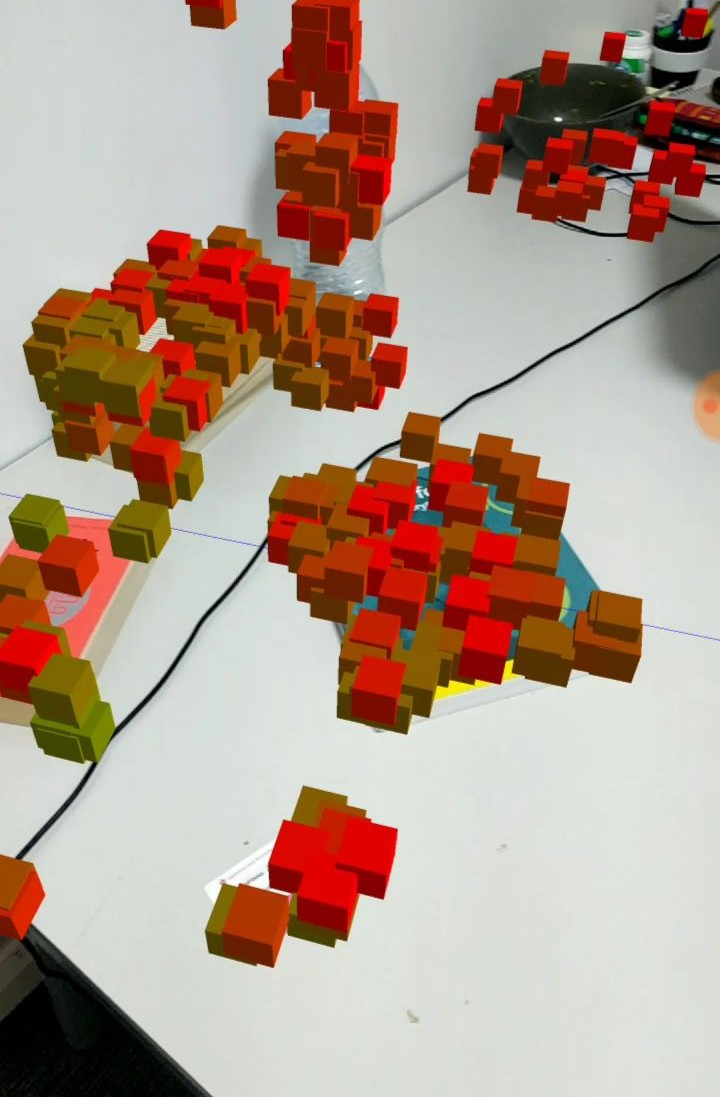
\includegraphics[height=8cm]{graphics/snapshot-points.jpg}
    \caption{Visualization of the information saved in a snapshot. Visible are the pixel data of the image and the subset of tracking points that are saved, symbolized by the cubes. Red cubes report a low confidence, green cubes a high confidence. The confidence information is currently not persisted in the snapshots, but useful for debugging.}
    \label{fig:snapshot_data}
\end{figure}

% - pipeline reports back with 2d PoI
% - challenge: likely won't have depth component for an arbitrary point on image
% - solution: project tracking points to 2d plane, find closest
When the data exploitation subsystem has established what the points of interest in the picture of a snapshot are, if any, it will instruct the snapshot to map their two-dimensional location on the picture back to a three-dimensional point in the virtual game space.
Due to the nature of the tracking points only appearing in segments of the picture that contain many features, we do not have the depth coordinate value for an arbitrary point on the image.
However, most of the time, we will have multiple tracking points close by, as points of interest are often found in areas with a lot of distinct objects, that is, not just a white wall, but for example characters on a piece of paper or a brand logo.
To solve the problem of lack of depth information, we make the assumption that any point that is as close as possible will suffice for our use case, since the 3D point is only used to direct our demon to the general area of the point of interest, in order to also lure the player to that same point.
As such, we simply project all 3D tracking points onto the 2D plane of our picture using the virtual camera's view-projection and select the corresponding 3D point of the closest point in 2D space as our point of interest in the virtual space.

% - pipeline calls project method, stores best hits for PoI
% - game/AR component later requests best 0-5 PoI from pipeline
% - generates random ones within room at reachable height to make game experience more consistent (i.e. not make game easier in plain rooms)
After projecting its 2D points of interest to 3D points, the data exploitation subsystem will store these points along with a score.
When the game informs the data exploitation subsystem that the scanning phase is over and we need to move to the capturing phase, the data exploitation subsystem will select those points with the highest score and provide them to the AR subsystem.
The AR subsystem will then select between three and five points for the route of the demon during the capturing phase.
If too little points were provided, the AR subsystem will generate additional points based on its current understanding of the room.
This ensures that the game experience will appear coherent, independent of the output of the exploitation subsystem.


\section{Data Analysis Implementation}

The major part of the data analysis is done in the scanning phase by the pipeline which can be seen in \autoref{fig:pipeline_phase1}.
The pipeline is started as soon as the AR subsystem hands over as snapshot.
In addition to the features described in \autoref{sec:snapshots} a score is added to the snapshot to determine its quality.
Furthermore, an offset will be tracked if the original frame will be cropped and only a small part is used for further processing. \\
Every snapshot will then be analyzed with the intent to minimize the traffic between the client and the server by sending only the best frames.
The server-side analysis will then yield points of interest based on those frames.

\begin{figure}[ht]
    \centering
    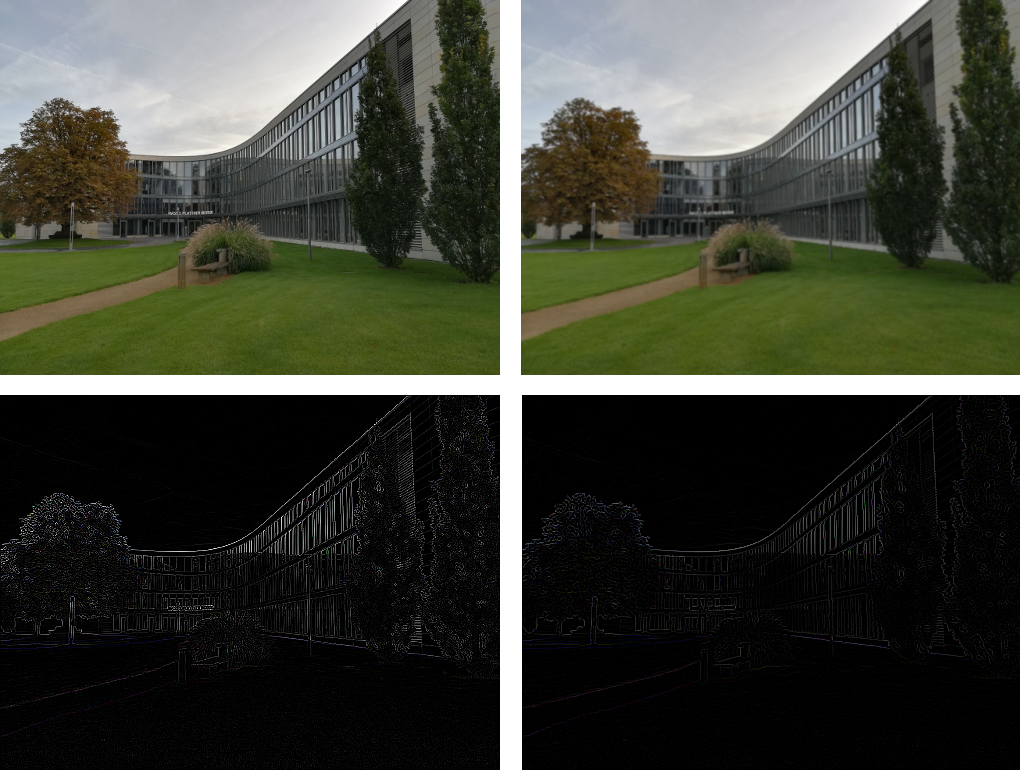
\includegraphics[width=8cm]{graphics/blur_grid_sep.png}
    \caption{Sharp images (with and without Laplace operator) on the left and analogous blurry images on the right}
    \label{fig:blur_estimation}
\end{figure}

\begin{figure*}[t]
  \centering
  \subcaptionbox{Original  input frame.\label{fig:cont_dect1}}[.3\linewidth][c]{%
    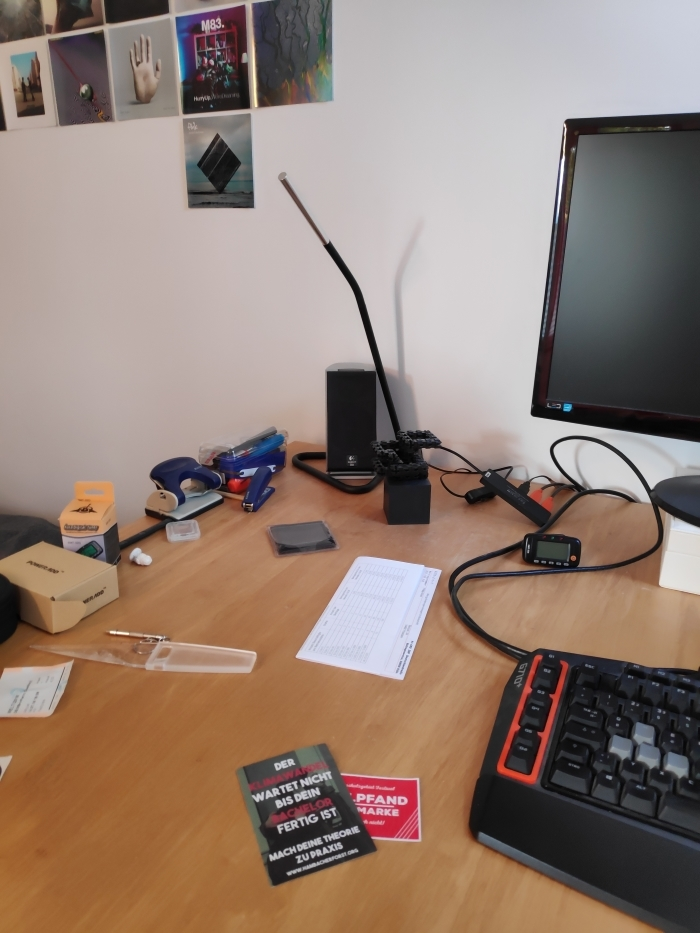
\includegraphics[height=7.2cm]{graphics/contours/original.jpg}}\quad
  \subcaptionbox{Preprocessed and binarized  frame.\label{fig:cont_dect2}}[.3\linewidth][c]{%
    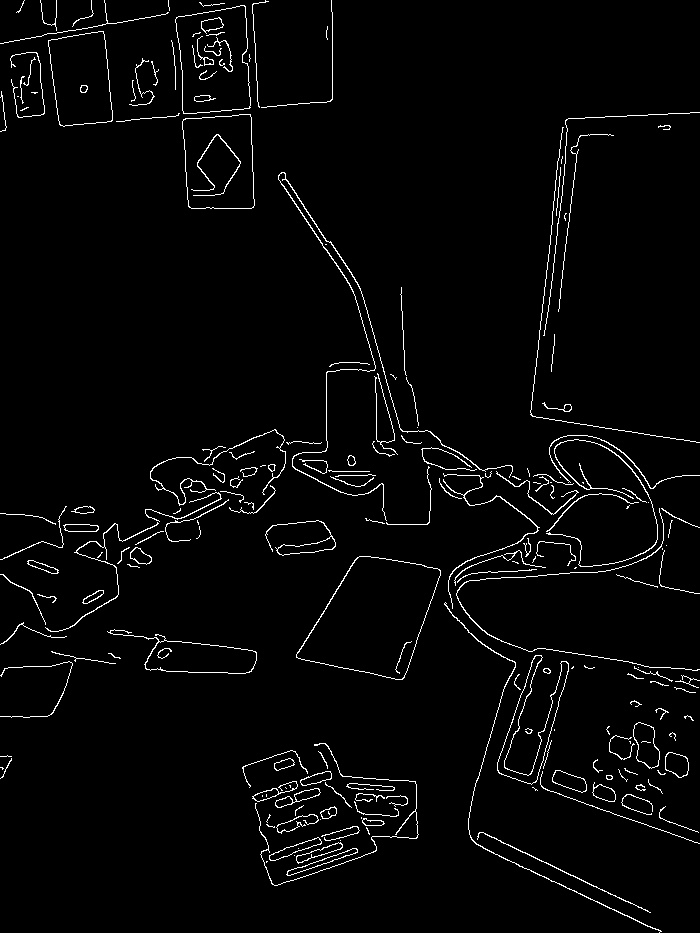
\includegraphics[height=7.2cm]{graphics/contours/canny.jpg}}\quad
  \subcaptionbox{Selected contours, passing contours are marked in green.\label{fig:cont_dect3}}[.3\linewidth][c]{%
    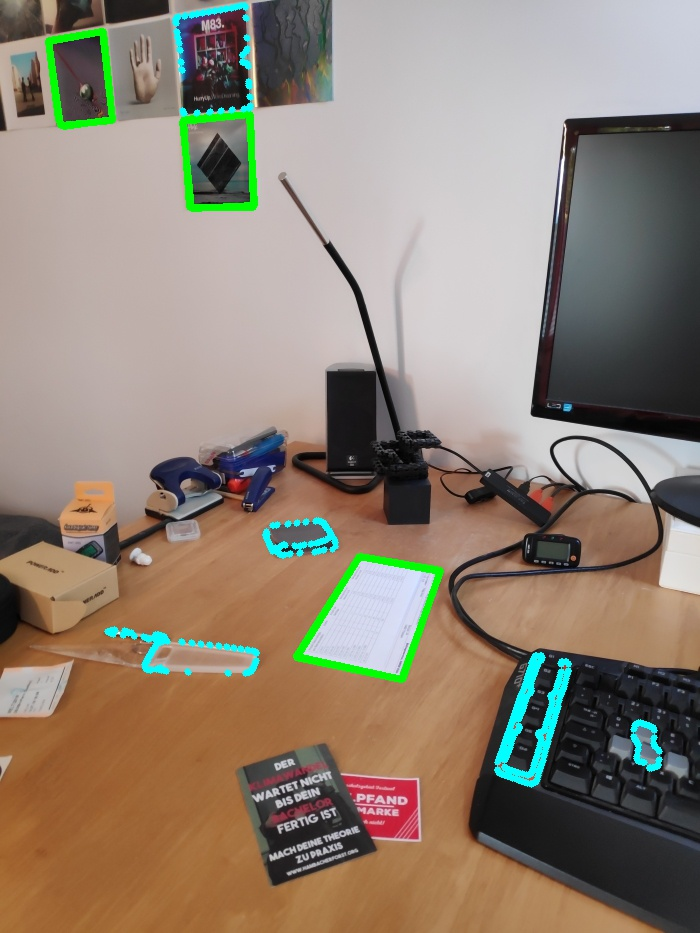
\includegraphics[height=7.2cm]{graphics/contours/finished.jpg}}

  \caption{Detection of contours in a real-word scene.}\label{fig:cont_dect}
\end{figure*}

\subsection{Steps}

The \emph{step} object is the abstract representation of each possible step of the pipeline and therefore each implementation provides the same interface to ensure interchangeability and reusability.
After a step is executed via calling the \emph{start} function the \emph{process} method is called and will, as the name implies, do the actual processing of a frame.
Afterward, the \emph{output} method will start all its following steps with the possibly new snapshot.\\
A special case of a step is the \emph{StepWithQueue} class where each snapshot is put into a priority queue based on its score.
This is useful in cases where only the best frame should be processed or where it should be processed first.
In this section we will explain the specific steps used in the scanning phase pipeline shown in \autoref{fig:pipeline_phase1} in detail.
% Daten-Analyse-Pipeline
 % Finden von PoI
 % Capturing und Processing
 
 
\textbf{Blur Estimation: } 
The first step of the pipeline is needed to preselect snapshots of which the quality is sufficient for further processing. 
The frame of the snapshot, which is processed, will be converted to a grayscale image before the Laplace operator is applied to it.
Examples of possible results after applying the Laplace operator can be seen in \autoref{fig:blur_estimation}.
Afterward, the variance of the new image will be calculated and will indicate the blurriness where a higher variance will represent a sharper image.
The idea behind this approach is that a blurry image (because of its nature) is less likely to have a lot of clear edges. 
Therefore the variance of the Laplace operator, which is used to detect edges, will be lower than in a sharp picture. 
For instance, the variance of the sharp picture displayed in \autoref{fig:blur_estimation} has a variance of 1152, whereas the variance of the blurry one is only 7. 
 
 \textbf{Angle Change: }
Subclassing from \emph{StepWithQueue}, the Angle Change Step won't process each snapshot individually but rather place them in a priority queue.
Only when the phone has been moved more than 10 centimetres in any direction or has been rotated by more than 5 degrees the best snapshot will be passed to the next steps.
Eventually, the queue will be cleared of all the remaining snapshots.
 
\textbf{Pattern Recognition: }
One of our assumed use cases for the game-based object detection is the recognition of known patterns, for example brand logos or in more extreme cases symbols that show dissident tendencies.
This is a classic use case for a feature matching approach.
We utilize an ORB (Oriented FAST and Rotated BRIEF) key point descriptor described by Rublee et al. that is rotation invariant and robust to noise, and therefore well applicable to real-world scenes~\cite{rublee2011orb}.
In the initialization of this step, the descriptors for all input logos are calculated and stored for later comparison.
When a frame enters the step, key points are calculated and compared to the known logos with a brute force matcher using a hamming distance as the measurement.
Every pairing falling under a fixed threshold is considered a match, and the mobile client sends a sighting confirmation to the data backend.
We were able to choose this threshold in a way that false positives were nonexistent in our tests, while still providing a satisfying match rate.
As the descriptor calculation for the frame takes around a hundred times longer than the actual matching with a comparison image, we can search for a large number of logos before performance concerns become relevant.
The brand matching use case, therefore, does not rely on computationally expensive machine learning models.


% \begin{figure}%
%     \centering
%     \subfloat[Frame input\label{fig:cont_dect1}]{{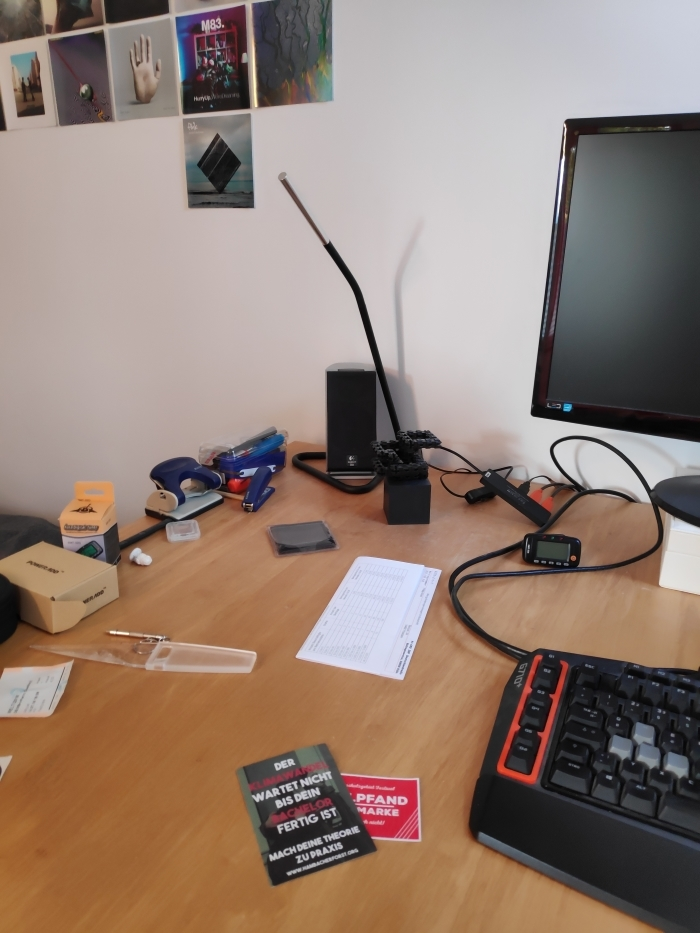
\includegraphics[height=7.2cm]{graphics/contours/original.jpg}}}%
%     \qquad
%     \subfloat[Preprocessed frame\label{fig:cont_dect2}]{{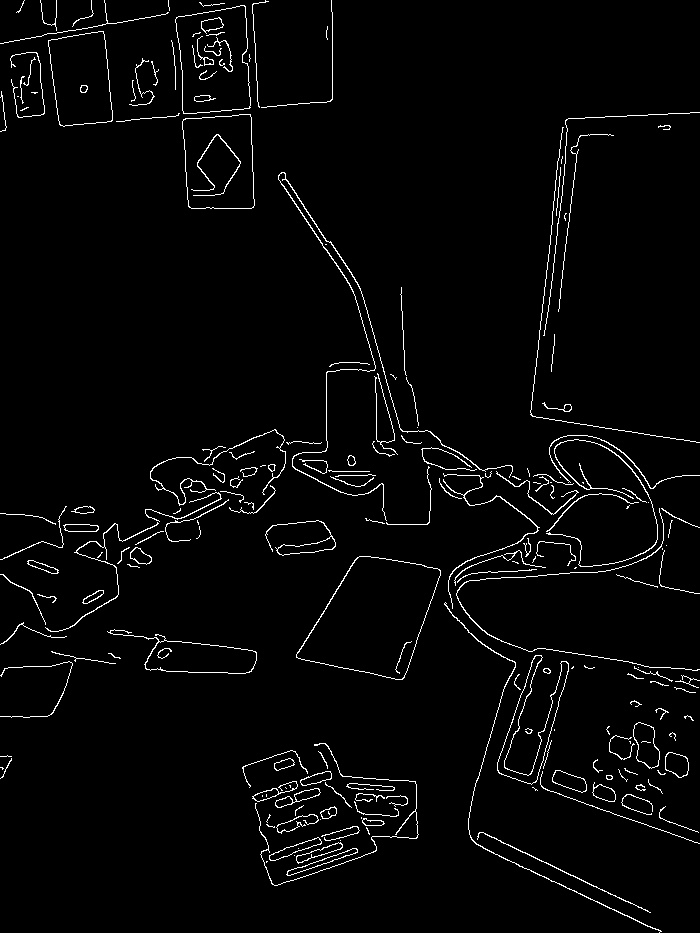
\includegraphics[height=7.2cm]{graphics/contours/canny.jpg}}}%
%     \qquad
%     \subfloat[Selected contours\label{fig:cont_dect3}]{{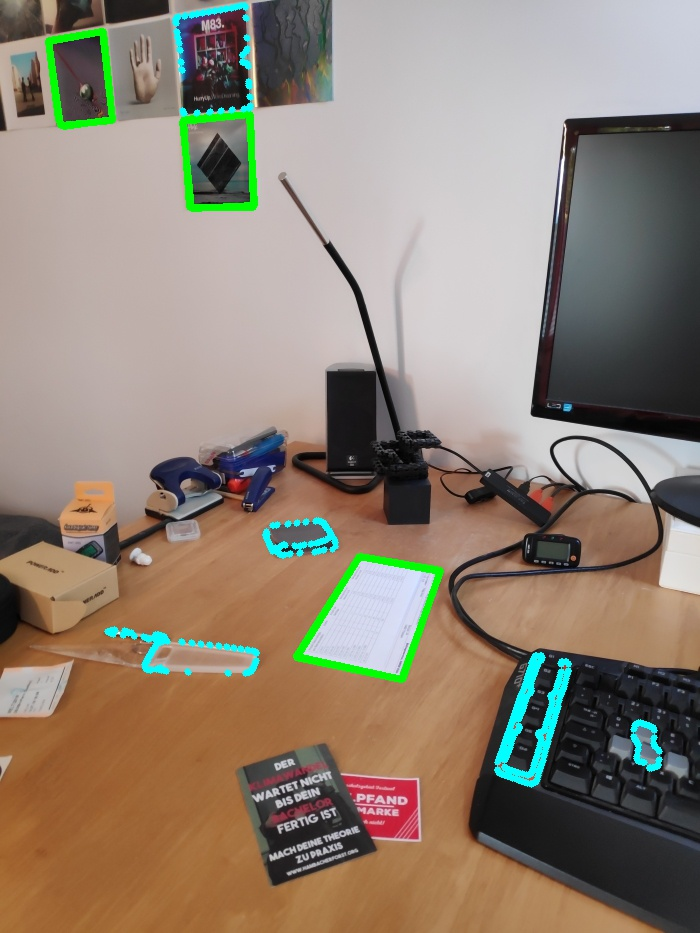
\includegraphics[height=7.2cm]{graphics/contours/finished.jpg}}}%
%     \caption{Detection of contours in a real-word scene.}%
%     \label{fig:cont_dect}
% \end{figure}
\textbf{Contour Detection: }
As a starting point to check areas of the incoming frame for potentially sensitive information, we detect contours in the scene.
We reason that this information can most likely be found in areas discernible from the rest of the frame, for example, a piece of paper.
The frame is preprocessed in several steps to maximize recognizable contours:
First, we apply a Gaussian Blur with a small kernel to reduce image noise, and then apply a bilateral filter to smooth the image further while keeping edges intact.
Afterward, a Canny edge filter with a dynamic threshold is applied to binarize the frame.
The result of this preprocessing can be found in \autoref{fig:cont_dect1}.
On this image, we run a contour detection algorithm provided by OpenCV to retrieve a list of contours.
Contours with a small size beneath a fixed threshold are culled from this list to further sort out \enquote{scene noise} like the numerous objects on the left side of the desk.
The outlines of these contours are approximated by polygons for which the deviation epsilon is based on the contour's area.
Once again we sort out polygons with more than seven edges to reduce our set of candidates.
All contours with a large enough area can be seen in \autoref{fig:cont_dect3}. Those with simple enough approximations are colored green.
We can see that from the complex original scene, only three areas of the image remain.
However, one potentially interesting area in the foreground is left out and thus will not be considered in later steps of the pipeline.
Each selected contour is cropped from the image and will be passed forward to the next step.

\textbf{Noise Estimation: }
To determine which of the found contours are likely to contain (textual) information, we first calculate a noise measure.
We use a simple kernel for fast noise variance estimation proposed by Immerkaer.~\cite{immerkaer1996fast}.
The author notes that \enquote{In highly textured images or regions, though,
the noise estimator perceives thin lines as noise}.
We utilize this property of the estimator as a criterium for the detection of small, dense text.
Areas with a low noise value are discarded in this step.
It is, however, completely plausible that high-noise contours do not contain text.
The score of the snapshot is multiplied with the noise value, and if the noise threshold is passed, the snapshot is passed on to the next step.

\textbf{Colorfulness Estimation: }
To further preselect the remaining contours, we estimate the colorfulness of the image regions.
A fast method for this is proposed by Hasler, meant to be used as an overall colorfulness estimation of a natural scene.~\cite{hasler2003measuring}.
We presume that regions of legible text are usually low in color variance to increase the contrast between letters and background.
Regions with high color variance are therefore not passed forward to the next step.
The score is once again multiplied with the colorfulness value.
In practice, contours with a high amount of noise and a low color variance are good estimates for regions of the image that actually contain text.
The scores of the two estimation measures on the found contours and a piece of wall and desk for comparison's sake can be seen in \autoref{fig:estimators}.
We can see that the letter does indeed possess a high noise score, but the colorfulness is not especially different from the other low-color contours.
We therefore send each contour passing the preselect steps to the data backend for further analysis of scene text occurrences.

\begin{figure}[t]
\centering
  \subcaptionbox{\textbf{N:} 0.9, \textbf{C:} 11.9\label{fig:estimators1}}{%
    
\includegraphics[height=3cm]{graphics/estimators/cover1.jpg}}\quad
  \subcaptionbox{\textbf{N:} 0.95, \textbf{C:} 15.5\label{fig:estimators2}}{%
    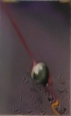
\includegraphics[height=3cm]{graphics/estimators/cover2.jpg}}\quad
  \subcaptionbox{\textbf{N:} 1.29, \textbf{C:} 13.1\label{fig:estimators3}}{%
    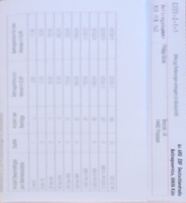
\includegraphics[height=3cm]{graphics/estimators/letter.jpg}}
\newline
\centering
  \subcaptionbox{\textbf{N:} 0.6, \textbf{C:} 1.8\label{fig:estimators4}}{%
    
\includegraphics[height=2.5cm]{graphics/estimators/wall.png}}
  \subcaptionbox{\textbf{N:} 0.8, \textbf{C:} 30.3\label{fig:estimators5}}{%
    
\includegraphics[height=2.5cm]{graphics/estimators/desk.png}}

  \caption{Noise (N) and Colorfulness (C) estimators applied to dewarped contours and wall and desk textures for comparison.}\label{fig:estimators}
\end{figure}

\subsection{Communication Between Phone and Server}

After a snapshot was processed in the pipeline it is added to the priority queue of the sending step where all snapshots are ordered by their calculated score.
The transmission itself is handled by \emph{Volley} a fast Android networking library~\cite{volley}.
Every 0.5s a POST-request will be prepared including the base64 encoded frame of the best snapshot in the priority queue and the id of the player. 
After being added to the request queue of Volley, the request will then be sent to the \emph{detect\_text} endpoint of the server as soon as possible.

Additionally, every 100th frame, which enters the pipeline will be added to the queue of the sending step directly after passing the blur estimation and angle change step.
This ensures that once in a while a data sent to the server if no other snapshot has a sufficient score after passing the other steps.
The score generation, however, guarantees that this very rarely the case.

In two special cases, requests are directly queued into Volley's request queue and avoid being processed in the sending step.
This is the case if a brand is successfully detected in the brand detection step or when the user successfully casts a spell in the demon capturing phase. 
In the first case, only the user id and the detected brand are transmitted as string whereas in the second one the full camera frame is transmitted alongside the user id.

\subsection{Server-side Analysis}

The backend is based on the Python framework \emph{Flask}~\cite{flask} and provides multiples endpoints where it accepts data sent from the Android Clients.

Frames that were processed in the scanning pipeline will be sent to the \emph{detect\_text} endpoint where a text detection will be applied.
A frame which passes the pipeline is likely to include text but to guarantee that this is the case and not only random noise was found, a text detection is applied. 
The \emph{EAST scene text detection} proposed by Zhou et al. determines quadrilateral shapes around possible text areas by feeding the supplied frame into a pre-trained neural network~\cite{Zhou2017EASTAE}.
If text is found, the server calculates the center of all found shapes and sends a response with the coordinates back to the client, where the snapshot can project these values into a three-dimensional real-world point of interest.

If a close-up of a point of interest is taken in the second game phase, it will be transmitted via the \emph{ocr} route. 
This will trigger a more precise analysis of the received frame involving the \emph{EAST scene text detection} and \emph{pytesseract}~\cite{pytesseract}, which is a Python wrapper for Google's OCR framework \emph{Tesseract}~\cite{tesseract}.
The text detection is applied to the frame and the resulting text boxes will be processed individually in the following steps.
First, the image is rotated to ensure that the text is aligned with the borders of the image.
Subsequently, the image is converted to grayscale as well as eroded and dilated in order to remove potential noise.
A bilateral filter is then applied to receive an image which is only black and white because an OCR algorithm will work best under those circumstances.
Finally, said OCR algorithm which is provided by \emph{pytesseract} will be applied to the image.
Because of the preprocessing, it tries to interpret the given image as a single line of text which is either English or German. 
The resulting string will be saved to an SQLite database \cite{sqlite} together with the user id of the Android client, the filename of the cropped text box and a timestamp.

The third and last endpoint is called \emph{brand} and is used to store the user id, timestamp and the name of a recognized brand in the database.

% Frontend?

%----------------------------------------------------------------
% Evaluation
%----------------------------------------------------------------

\section{Evaluation}
\label{sec:evaluation}

% AR-Komponente (Bewegung des Dämons, Werden die PoI’s wiedergefunden, etc.)
% - biggest challenge: ensuring that tracking points at PoI remain consistent as user approaches; old visual context is lost as they focus e.g. on a single part of the desktop --> might cause ARCore to recalc coordinate system (could have been nice to pause allocation of tracking points and rely on accelerometer, but ARCore does not support this)
\subsection{Tracking point accuracy}
The most important limitation for the augmented reality subsystem we encountered was the stability of tracking points in the virtual space. As described before, quick movement caused ARCore to lose track of many of the points and creating new ones, thus invalidating potentially crucial information about the room. Since the setting of the game encourages of feeling of hunting after the demon, quick movements are unfortunately an expected and potentially necessary part of the game. Further problems arose when the user moved closer towards a point of interest at which the demon was sitting. As they approach the point, a lot of points all around the room will "disappear" as the frame of the camera narrows in on the area of interest. This would not necessarily be a problem, however ARCore will constantly recompute the coordinate system and make considerable corrections to the origin when it loses important tracking information or gets a lot of new points in an area. Often, this had the effect of the demon getting farther and farther away from the player as they approach it, even though it appeared to be sitting at a constant position.

At the time of writing, ARCore does not expose an option to "freeze" the coordinate system. This functionality would have likely remedied our issues, if we froze the coordinate system when switching to the capturing phase, where stable positions are essential, and relied on the phone's accelerometer and picture data to move the camera in the existing virtual space. ARCore did not expose sufficient access to the lower level system for us to try this approach by ourselves, so we will either have to wait for its developers to add this functionality or use and modify an open source augmented reality framework to solve this specific use case.

% FIXME: to be tested further:
% - by defining anchors on the relevant tracking points, ARCore will ensure most of the time that objects remain within reach -- timeout and fallback to showing spell even though user is not close enough otherwise
As a workaround to this issue, we make use of the ARCore anchors, which will update and move around the coordinate system to try and make up for changes to the coordinate system's origin or scale. This helped most of the time to ensure that the demon will at least be within the activation distance for the capturing phase, but it still appeared to coast around the spot. To not block the game altogether when the demon "hides" in a wall, we added a timeout that will move the game onwards in the hope that the next point may be better.

\subsection{Demon movement}
% - movement of demon feels weird at start, as dimensions of room are unknown
The movement of the demon in our current implementation is simplistic and makes next to no use of advanced possibilities, like collision detection. This is mainly because the quality of the tracking points even for our room size estimation may vary greatly, so that we chose to use the simplest possible primitive volume in 3D space to reduce the chance of the demon getting locked within non-existing obstacles that have been formed by errors in the tracking point estimation.

% - placement of waypoints close to user confuse, but as they traverse the room and turn frequently it's hard to predict where they will be
Our concept of exploring the room size by encouraging the user to turn frequently at the start of the session, by making the room very small, may lead to some confusion as the demon appears to travel through impossible ways, for example through the user.As the room quickly grows bigger, this may not be as much of an issue, however it may make sense to add a better waypoint system than simply selecting random points in the known space. This may also help to make the demon feel like a more believable creature.

\subsection{User experience}
% FIXME: to be evaluated if that applies to anyone else but me:
- handling of phone is tricky: most users held phone in right hand, shot w/ left hand in scanning phase. switch hands when entering capturing phase for drawing spells --> messes up coordinate system as phone points to floor temporarily

% Erkennung der Points of Interest
- Blurriness: Laplacian is not too precise, e.g. when using shallow focus, some regions are completely focused whereas some are totally blurry
--> will result in low blurriness value

% Brand-Detection

% Textanalyse mit OCR
- Wo wird im Bild Text erkannt?
- Kann dieser Text interpretiert werden, wenn ja, wie gut?
- Was sind Probleme? (Schriftart, Blurriness, distortion)

% Scalability



%----------------------------------------------------------------
% Conclusion
%----------------------------------------------------------------
\section{Conclusion}
\label{sec:conclusion}

As we have demonstrated, a system that continuously spies on the user while they are playing an augmented reality game is feasible to build, especially with the prospect of our employed frameworks being continuously improved. We also showed how a preprocessing on the client allows reducing the amount of data that is actually communicated to the server to a minimum, thus disguising the illicit behavior from the user. Even though a close analysis of the traffic of the application may reveal surprisingly frequent communication with a server, a more elaborate gameplay system incorporating real-time player-vs-player might be able to sell this as necessary as well.

As such, we believe that augmented reality applications may pose a great risk to the consumer. 
This makes it even more important than ever to take care when installing apps and only rely on those which are distributed by trusted sources such as the Google Play Store and Apple's App Store. \\
Additionally, users should always look out for suspicious behavior of apps, for example, if an app uses more permissions than needed for the basic functionalities, transfers lots of data via the Internet or requires a lot of CPU power.
An app is, however, still a black box to the users which will make it impossible for them to clearly separate malicious behavior from badly implemented apps.\\
Unfortunately, to this day there is no perfect protection against the kind of unwanted behavior which is outlined in this paper because a well made malicious app will always be able to hide its intents properly.


% Future Work
- z.B. weitere Daten sammeln und komplexere Nutzerprofile anlegen
- Data Analytics auf den gesammelten Infos

%----------------------------------------------------------------
% Sources
%----------------------------------------------------------------
\bibliographystyle{acmsiggraph}
\bibliography{foo-paper}
%\printbibliography 

\end{document}
